\section{Modelo macroeconométrico}
\label{Modelo_empirico}

\subsection{Investimento residencial e a taxa própria de juros dos imóveis}
\label{SecTxPropria}

O objetivo desta subseção é detalhar a relação entre investimento residencial e a taxa própria de juros dos imóveis desenvolvida por \textcite{teixeira_crescimento_2015} para então expor as hipóteses testadas no modelo econométrico.
Para evidenciar esta relação, deflaciona-se a taxa de juros hipotecárias pela inflação de imóveis tal como na equação \ref{tx_Propria}.
O gráfico \ref{gZ_Propria} ilustra como  este deflacionamento é mais adequado do que por um índice geral de preços ---  \textcite[p.~143--146]{fair_macroeconometric_2013} --- para captar a dinâmica do investimento residencial.
Destaca-se também que em momentos de especulação (\textit{i.e.} bolha de ativos, neste caso, imóveis) é a inflação destes ativos que domina a dinâmica da taxa própria \cite[p.~53]{teixeira_crescimento_2015}. Sendo assim, quanto menor esta taxa maiores serão os ganhos de capital (em imóveis) por se especular com imóveis.
Tal dinâmica é evidenciada no gráfico \ref{gZ_Propria} em que a taxa própria se reduziu progressivamente ao longo do \textit{boom} imobiliário (2002-5).


%TODO Alterar imagem


\begin{figure}[H]
	\centering
	\caption{Taxa real e própria de juros dos imóveis x investimento residencial}
	\label{gZ_Propria}
	\includegraphics[width=0.75\textwidth]{../../Dados/Fatos_Estilizados/figs/TxPropria_Investo.png}
	\caption*{\textbf{Fonte:} U.S. Bureau of Economic Analysis, elaboração própria}
\end{figure}

De modo a testar a capacidade explicativa da taxa própria para o investimento residencial, assume-se a seguinte relação de longo prazo tal como em \textcite{teixeira_crescimento_2015}:

\begin{equation}
g_{Z_t} = \phi_0 - \phi_1\cdot own_t
\end{equation}
sendo assim, se as séries forem cointegradas, é possível estimar um VECM nos seguintes termos:
\begin{equation}
\begin{cases}
\Delta own_t = \delta_{1} + \alpha_1(g_{Z_{t-1}} - \phi_0 + \phi_1\cdot own_{t-1}) + \sum^{N=4}_{i=1}\beta_{1,i}\cdot \Delta g_{Z_{t-i}} +
\sum^{N=4}_{i=1}\gamma_{1,i}\cdot \Delta own_{t-i} +\varepsilon_{t,1}
\\
\Delta g_{Z_{t}} = \delta_{2} + \alpha_2(g_{Z_{t-1}} - \phi_0 + \phi_1\cdot own_{t-1}) + \sum^{N=4}_{i=1}\beta_{2,i}\cdot \Delta g_{Z_{t-i}} +
\sum^{N=4}_{i=1}\gamma_{2,i}\cdot \Delta own_{t-i} +\varepsilon_{t,2}
\end{cases}
\end{equation}
em que $\delta_s$ indicam tendência linear nas respectivas séries em nível;
$\alpha_{is}$ são os coeficientes de correção de erro; 
$\beta_s$ e $\gamma_s$ são coeficientes associados as defasagens de  $g_Z$ e $own$ respectivamente e; $\varepsilon_s$ são os resíduos.
Seguindo as hipóteses de \textcite{teixeira_crescimento_2015}, os resultados esperados a serem testados são:
\begin{enumerate}
	\item $\varepsilon \sim I(0)$: Estacionariedade dos resíduos indica que taxa própria e $g_Z$ são cointegrados, ou seja, apresentam uma dinâmica de longo prazo em comum;
	\item $\alpha_1 = 0$: $own$ exogenamente fraca em relação ao $g_Z$;
	\item $\alpha_2 < 0$: Taxa própria causa (no sentido de Granger) investimento residencial;
	%TODO Checar sinal de alpha2
	\item $\phi_1 > 0$: $gZ$ e Taxa própria apresentam uma dinâmica negativa no longo prazo;
	\item $\phi_0 < 0$: Demanda por imóveis por motivos não-especulativos e associados a especificidades institucionais é estatisticamente significante e não-negativo;
	\item $\gamma_{2,is} < 0$: Taxa própria afeta o investimento residencial negativamente no curto prazo;
	\item $\beta_{1,is}$ = 0: Efeito do investimento de $g_Z$ sobre a taxa própria não é estatisticamente significante.
\end{enumerate}
Apesar de lançar luz sobre algumas relações relevantes esta proposição não foi avaliada por meio da estimação de um modelo macroeconométrico e isso será feito a seguir.

\subsection{Estimação do modelo}

O modelo a ser estimado pretende testar se a inflação de ativos (\textit{i.e.} inflação do preço dos imóveis) contribui para explicar a dinâmica do investimento residencial tal como proposto por \textcite{teixeira_crescimento_2015}. 
Vale relembrar que a seleção do período analisado decorre de quebras estruturais (ver tabela \ref{structbreak}) associadas às mudanças institucionais no-pós crise dos \textit{savings and loans} (FDIC e FIRREA).
Dito isso, foram utilizadas séries trimestrais com ajuste sazonal de 1992 a 2019 (ver gráfico \ref{YeoJhonson}) da taxa de juros das hipotecas fixas em trinta anos (MORTGAGE30US, trimestralizada pelo fim do período), investimento residencial (PRFI, em taxa de crescimento) e índice de Case-Shiller (CSUSHPISA, trimestralizada pelo fim do período). 

Por se tratar de taxas de crescimento com ampla volatilidade, aplicou-se a transformação de \textcite{yeo_new_2000} para conter a amplitude das séries decorrente da crise imobiliária. A razão de se utilizar tal procedimento e não a transformação de \textcite{box_analysis_1964} é por não se restringir a valores não-negativos. Em seguida, foram realizados testes de raiz unitária (tabela \ref{unitroot}) bem como o procedimento de \textcite{johansen_estimation_1991} (tabela \ref{Johansen}) e, a um nível de significância de 5\%, conclui-se que as séries são cointegradas e, portanto, um modelo do tipo vetor de correção de erros (VECM) é a melhor forma de estimação para este caso \cite{enders_applied_2014}.


\input{./Fatos_Estilizados/Quebra.tex}

\input{./Fatos_Estilizados/Raiz.tex}

% Please add the following required packages to your document preamble:
% \usepackage{multirow}
% \usepackage{graphicx}
\begin{table}[htb]
\centering
\caption{Teste de cointegração}
\label{Johansen}
\begin{threeparttable}
%\resizebox{\textwidth}{!}{%
\begin{tabular}{l|l|cc}
\hline
 \hline
\multirow{2}{*}{\textbf{Modelo}} & \multirow{2}{*}{\textbf{Hipótese}\tnote{a}} & \multicolumn{2}{c}{\textbf{Procedimento de Johansen}} \\ \cline{3-4} 
 &  & \multicolumn{1}{c|}{Estatística} & valor crítico (5\%) \\ \hline
\multirow{3}{*}{\textbf{$g_Z$, Taxa Própria}\tnote{b}} & $r = 0$ &20.13&19.96\\
 & $r = 1^*$ &3.57&9.24\\\hline	
\multirow{4}{*}{\textbf{$g_Z$, Inflação e Juros}\tnote{c}} & $r = 0$ &44.34&34.91\\
 & $r = 1$ &26.22&19.96\\
 & $r = 2$ &10.69&9.24\\\hline
\multirow{3}{*}{\textbf{$g_Z$, Inflação e Juros exógeno}\tnote{d}} & $r = 0$ &36.96& 19.96\\ 
 & $r = 1^*$ &8.03&9.24\\ 
  \hline
\end{tabular}%
%}
\footnotesize{(a) Utilizado teste do traço com constante e defasagem selecionada a partir do critério AIC. (b) Testado para o lag 5. (c) Testado para o lag 5. (d) Testado para o lag 5. (*) Indica que o \textit{rank} selecionado implica em cointegração.}
\end{threeparttable}
\caption*{\textbf{Fonte:} Elaboração Própria}
\end{table}

%TODO Alterar figura
\begin{figure}[H]
	\centering
	\caption{Séries com transformação de \textcite{yeo_new_2000}}
	\label{YeoJhonson}
	\includegraphics[width=\textwidth]{../../Dados/Fatos_Estilizados/figs/YeoJohnson_All.png}
	\caption*{\textbf{Fonte:} U.S. Bureau of Economic Analysis, elaboração própria}
\end{figure}


Dito isso, resta determinar a defasagem utilizada. Pelos critérios de informação, tanto o primeiro (trimestre) quanto o quarto \textit{lag} são elegíveis (ver tabela \ref{criterios}). Apesar de parcimonioso, a escolha da primeira defasagem não possui respaldo empírico. Se considerar o tempo médio de construção de imóveis desde a aprovação até a conclusão, verifica-se que deve-se incluir \textit{ao menos} o segundo \textit{lag} para incorporar as residências construídas para a venda uma vez que tal motivação só é realizada se concluída a construção (ver figura \ref{meses}). Tal procedimento, no entanto, não é suficiente para determinar a seleção do \textit{lag} a ser utilizado. Dado que o fluxo de novos imóveis é significativamente inferior ao estoque existente, o efeito da variação dos preços se verifica mesmo com as construções não concluídas, ou seja, impacto decorre das residências concluídas anteriormente.  Tal elemento seria captado pela taxa própria \textit{esperada}. No entanto, não há uma série para tal de modo que as defasagens são uma primeira aproximação para a taxa esperada.


\begin{table}[htb]
	\caption{Seleção da ordem do VECM (* indica o mínimo)}
	\label{criterios}
\begin{center}
\begin{tabular}{lcccc}
\toprule
            & \textbf{AIC} & \textbf{BIC} & \textbf{FPE} & \textbf{HQIC}  \\
\midrule
\textbf{0}  &      -16.26  &     -15.99*  &   8.680e-08  &       -16.15   \\
\textbf{1}  &      -16.23  &      -15.85  &   8.915e-08  &       -16.08   \\
\textbf{2}  &      -16.35  &      -15.87  &   7.902e-08  &       -16.16   \\
\textbf{3}  &      -16.39  &      -15.80  &   7.604e-08  &       -16.15   \\
\textbf{4}  &     -16.49*  &      -15.79  &  6.909e-08*  &      -16.21*   \\
\textbf{5}  &      -16.43  &      -15.61  &   7.389e-08  &       -16.10   \\
\textbf{6}  &      -16.38  &      -15.46  &   7.737e-08  &       -16.01   \\
\textbf{7}  &      -16.32  &      -15.29  &   8.253e-08  &       -15.91   \\
\textbf{8}  &      -16.32  &      -15.18  &   8.297e-08  &       -15.86   \\
\textbf{9}  &      -16.26  &      -15.01  &   8.898e-08  &       -15.75   \\
\textbf{10} &      -16.24  &      -14.89  &   9.084e-08  &       -15.69   \\
\textbf{11} &      -16.47  &      -15.01  &   7.260e-08  &       -15.88   \\
\textbf{12} &      -16.41  &      -14.84  &   7.815e-08  &       -15.77   \\
\textbf{13} &      -16.38  &      -14.71  &   8.060e-08  &       -15.71   \\
\textbf{14} &      -16.34  &      -14.55  &   8.546e-08  &       -15.62   \\
\textbf{15} &      -16.29  &      -14.39  &   9.119e-08  &       -15.52   \\
\bottomrule
\end{tabular}
%\caption{VECM Order Selection (* highlights the minimums)}
\end{center}
\caption*{\textbf{Fonte:} Elaboração própria}
\end{table}


\begin{figure}[H]
	\centering
	\caption{Tempo médio de construção (aprovação a conclusão) de imóveis para uma unidade familiar por propósito de construção exceto casas pré-fabricadas (1976-2018)}
	\label{meses}
	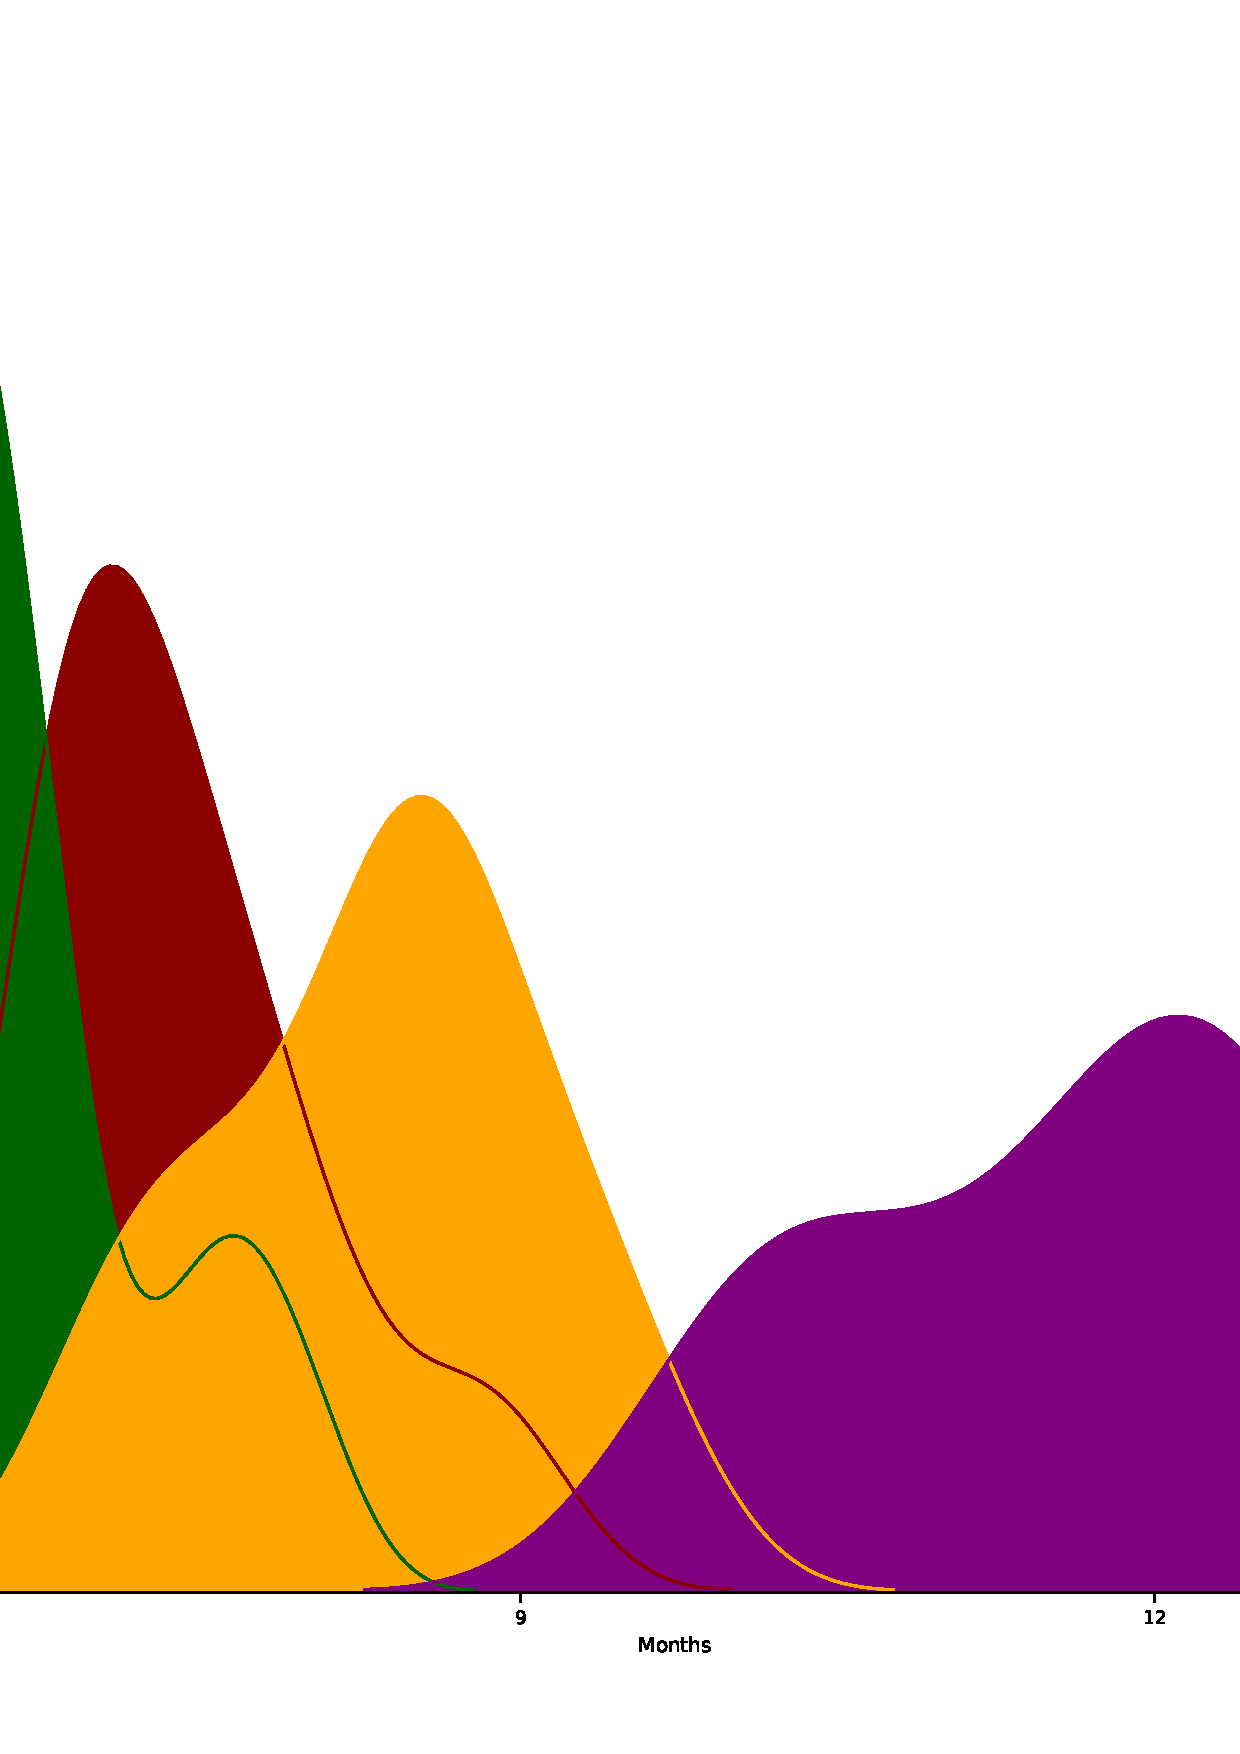
\includegraphics[width=\textwidth]{Fatos_Estilizados/Figs/Meses_contrucao.png}
	\caption*{\textbf{Fonte:} Survey of Construction (SOC), elaboração própria}
\end{figure}

Desse modo, uma alternativa é por meio de uma ``teoria prática do futuro'' --- como em \textcite[p.~214]{keynes_general_1937} --- em que o processo decisório para iniciar a construção de um novo imóvel depende de componentes expectacionais/convenções associados as observações passadas.
De forma a ilustrar tal relação, o gráfico \ref{defasagens} apresenta as variáveis de interesse frente ao \textit{lag} que minimiza os critérios de informação. Esse procedimento permite visualizar se existe alguma relação entre a taxa própria esperada (taxa efetiva defasada) e taxa de crescimento do investimento residencial\footnote{De modo a dar conta de não-linearidades, é apresentada a regressão quadrática entre ambas as variáveis (e o mesmo foi realizado para o gráfico inverso).}. Já a relação inversa, qual seja, da taxa de crescimento para a taxa própria não se verifica uma vez que, como visto, o fluxo de novos imóveis é bastante inferior o estoque de imóveis existente e, portanto, é esperado que tal relação não esteja presente. Em outras palavras, a especulação com o \textit{estoque}  de imóveis gera inflação desses ativos que, por conseguinte, afeta a construção de novos imóveis (\textit{fluxo}) e não o inverso. 
%TODO Referência de terra ser escassa.
Essa inspeção, portanto, ilustra de forma bastante grosseira tal componente expectacional por meio da menor dispersão entre os pontos no gráfico inferior direito\footnote{Raciocínio semelhante pode ser encontrado em \textcite{girardi_autonomous_2015}}.  


\begin{figure}[htb]
	\centering
	\caption{Dispersão entre taxa própria e crescimento do investimento residencial: defasagens selecionadas a partir dos critérios de informação}
	\label{defasagens}
	\includegraphics[width=\textwidth]{../../Modelo/SeriesTemporais/figs/VEC_Defasagens.png}
	\caption*{\textbf{Fonte:} Elaboração própria}
\end{figure}
%TODO Adicionar gráficos com defasagem 2


\begin{figure}[H]
	\centering
	\caption{Inspeção dos resíduos da estimação}
	\label{residuos}
	\includegraphics[height=.4\textheight]{../../Modelo/SeriesTemporais/figs/Residuos_4VECM.png}
	\caption*{\textbf{Fonte:} Elaboração própria}
\end{figure}

\begin{table}[htb]
\centering
	\caption{Parâmetros da estimação (VECM)}
\input{./Fatos_Estilizados/Estimacao_VECM.tex}
\caption*{\textbf{Fonte:} Elaboração própria}
\end{table}

%TODO Modificar tabela da estimação

Feita esta contextualização teórica da escolha das defasagens,  estima-se um VECM de ordem 4\footnote{Nota-se que tal defasagem, além de ser teoricamente justificada, também gera resíduos não heterocedásticos e sem correlação serial (ver tabela \ref{testes_resduos}).} cujos resíduos são apresentados no gráfico \ref{residuos} e resultados são expostos na tabela \ref{Estimacao}\footnote{Os resultados de todos os testes realizados bem como as rotinas utilizadas estão disponíveis sob solicitação.}.
Começando pela relação de cointegração, verifica-se que é estatisticamente significante para ambas as equações de modo que as variáveis partilham uma relação (negativa) de longo prazo, ou seja, são cointegradas (fundamentando 1 e 4).
Desse modo, a proposição de \textcite{teixeira_crescimento_2015} é corroborada por meio do coeficiente $\phi_1> 0$ e estatisticamente significante.
Além disso, os coeficientes $\gamma_{2,is}$ estimados são negativos seguindo os resultados esperados (6) do mesmo modo que a demanda por imóveis por motivos não-especulativos ($\phi_0$) é estatisticamente significante (resultado 5).
Adotando um nível de significância de 5\%, verifica-se que o parâmetro de correção de erro é estatisticamente significante apenas para a equação da taxa de crescimento do investimento residencial. Portanto, $own$ é exogenamente fraca em relação a $g_Z$ enquanto taxa própria Granger-causa $g_Z$, validando os resultado esperados (2) e (3).
Já as relações de curto prazo entre taxa própria e $g_Z$ (capturadas por $\beta_{1,is}$) não são estatisticamente significantes a 5\% \footnote{O resultado esperado (7) também pode ser confirmado a partir da inspeção da tabela \ref{Estimacao} em que apenas a quarta defasagem da taxa própria é estatisticamente significante nesta equação.}. Em resumo, os resultados obtidos estão em linha com os esperados. 

Uma forma de verificar a capacidade explicativa da taxa própria para $g_Z$ é por meio da decomposição da variância da previsão (FEVD) como no gráfico \ref{fevd}\footnote{Também é importante destacar que dado o número de variáveis (duas), a ordenação de Choleski é suficiente para analisar a função resposta ao impulso uma vez que gera uma matriz semelhante a de um VECM estrutural. 
}. Verifica-se que desde o primeiro trimestre a taxa própria contribui para $g_Z$ enquanto o inverso não é válido. Adicionalmente, é notável que tal contribuição é crescente e maior que 50\% para além do 3º trimestre. Portanto, a taxa própria é explicada principalmente por ela mesma e explica $g_Z$ consideravelmente.

\begin{figure}[htb]
	\centering
	\caption{Decomposição da variância da previsão}
	\label{fevd}
	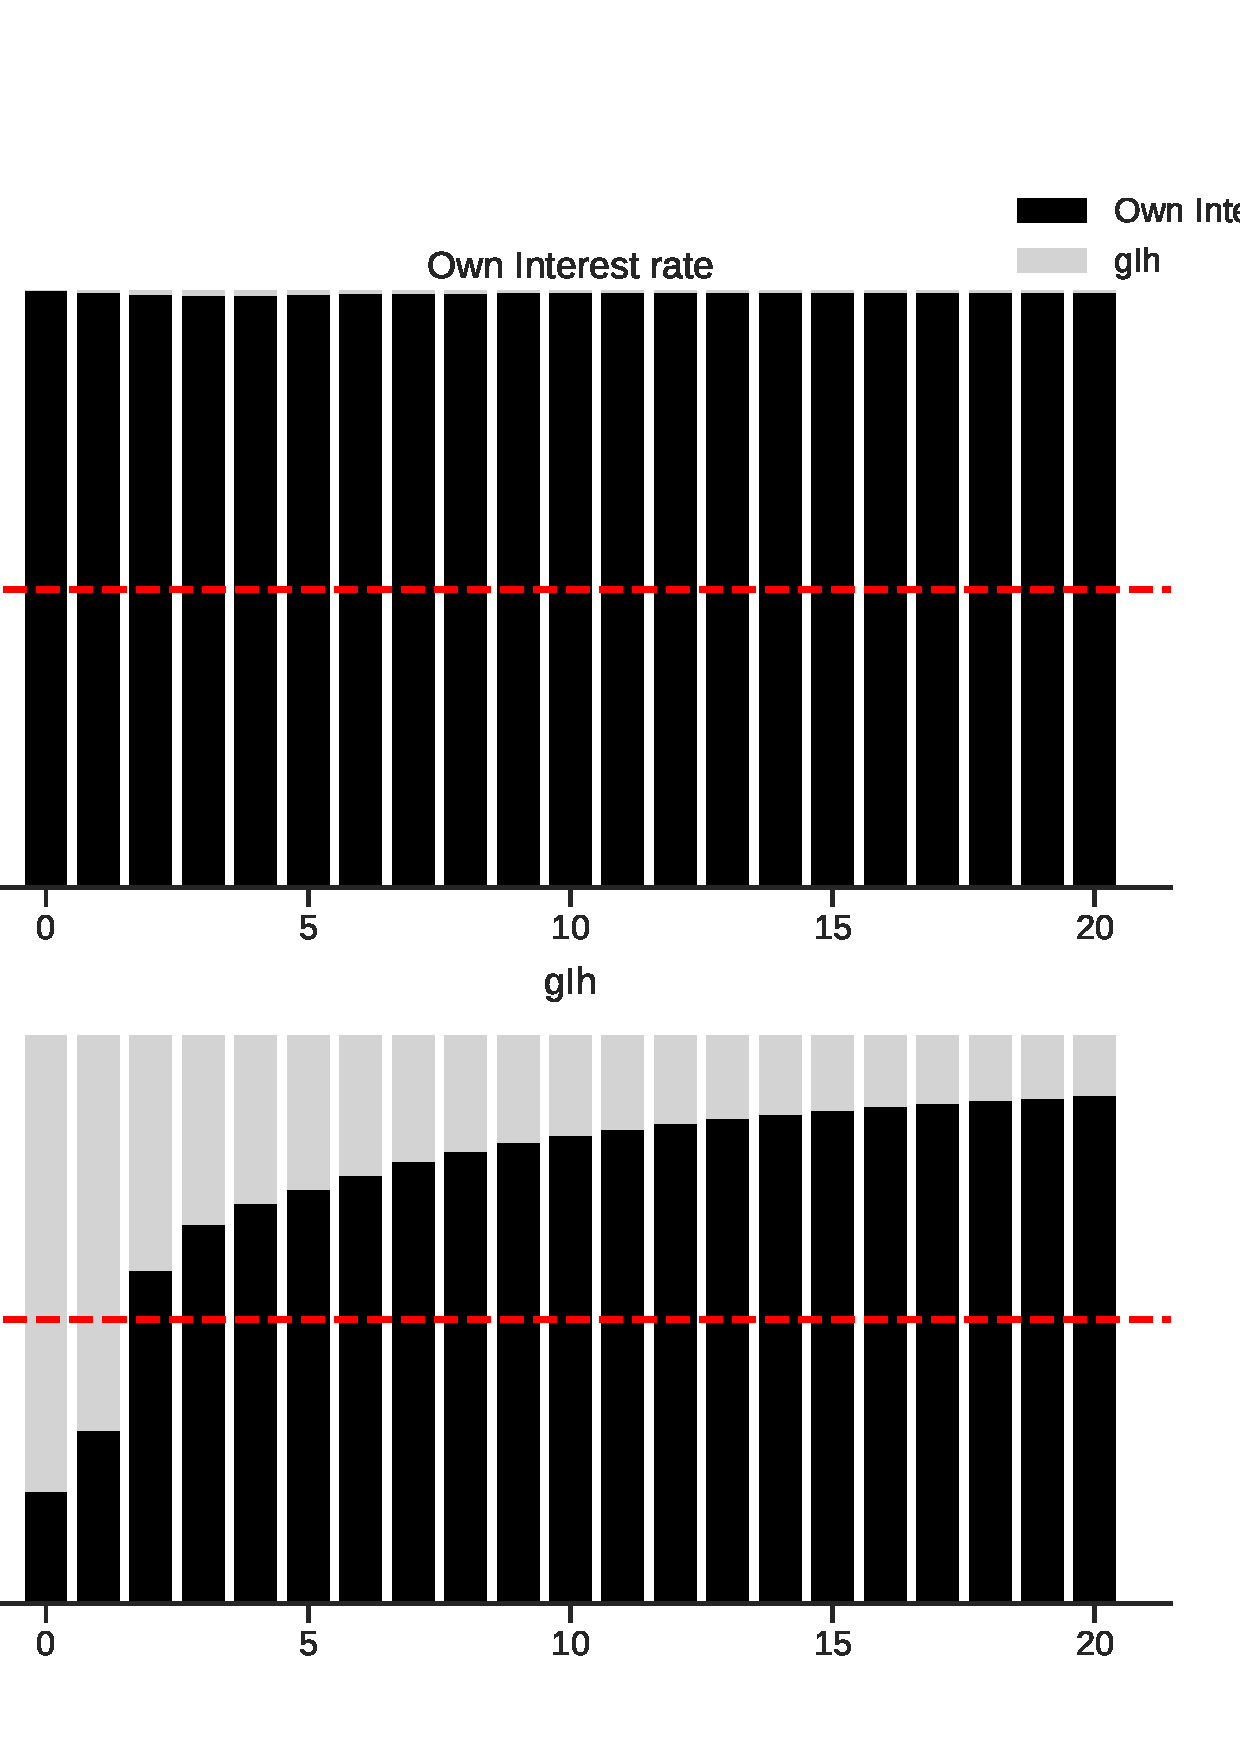
\includegraphics[width=\textwidth]{../../Modelo/SeriesTemporais/figs/FEVD_VECMpython_TxPropria.png}
	\caption*{\textbf{Fonte:} Elaboração própria}
\end{figure}


Adiante, é apresentado o gráfico da função impulso resposta ortogonalizada --- grosso modo, as conclusões da FEVD se estendem também para os choques --- em que são avaliados os impactos no aumento de um desvio-padrão em uma das variáveis endógenas no primeiro período apenas.
%TODO Checar
A partir deste gráfico, verifica-se que o sistema é estável uma vez que os efeitos do aumento de $g_Z$ sobre $g_Z$ é amortecido ao longo do tempo enquanto os efeitos da taxa própria sobre a ela mesma são persistentes mas não explosivos.
Já os efeitos de $g_Z$ sobre a taxa própria são nulos uma vez que o intervalo de confiança sempre abrange o zero. Por fim, e este é o resultado relevante, dados os objetivos, é o efeito negativo considerável e duradouro da taxa própria sobre $g_Z$, confirmando a tese de \textcite{teixeira_crescimento_2015}.
Em resumo, as funções resposta ao impulso indicam que o aumento da taxa de juros das hipotecas (aumento na Taxa Própria) impacta negativamente na taxa de crescimento residencial enquanto o aumento da inflação de ativos implica no inverso. 
%alinhado com os resultados de \textcite{huang_is_2018} para o longo prazo.
%podendo estar associado aos gastos com aprimoramento residencial uma vez encerradas as construções (também contabilizado como investimento residencial).


\begin{figure}[H]
	\centering
	\caption{Função impulso resposta ortogonalizada}
	\label{fevd}
	\includegraphics[width=\textwidth]{../../Modelo/SeriesTemporais/figs/Impulso_VECM.png}
	\caption*{\textbf{Fonte:} Elaboração própria}
\end{figure}

Dos resultados apresentados acima, verifica-se que a taxa própria de juros dos imóveis tem uma capacidade explicativa significativa. Vale destacar que apesar de amplitude das defasagens selecionadas, o modelo estimado é bastante parcimonioso em termos das variáveis utilizadas. Desse modo, considerando o grau de parcimônia e a robustez dos resultados, conclui-se que é um modelo satisfatório para explicar a taxa de crescimento do investimento residencial. 
%Diante da qualidade do ajuste, o gráfico \ref{previsao} apresenta a previsão do modelo 4 passos a frente. 
%Avaliando o últimos resultados disponíveis das contas nacionais e estimativas da taxa própria, verifica-se uma previsão satisfatória uma vez que tanto $g_Z$ reduz quanto a taxa própria aumenta.

\begin{comment}
\begin{figure}[H]
	\centering
	\caption{Previsão 4 passos a frente}
	\label{previsao}
	\includegraphics[width=\textwidth]{Fatos_Estilizados/Figs/Previsao_VECM.png}
	\caption*{\textbf{Fonte:} Elaboração própria}
\end{figure}


\begin{center}
\begin{table}[H]
\centering
\caption{Parâmetros para a equação da Taxa Própria}
\begin{tabular}{lccclcc}
\toprule
\textbf{Equação:} Taxa própria & \textbf{coef} & \textbf{std err} & \textbf{z} & \textbf{P$> |$z$|$} & \textbf{[0.025} & \textbf{0.975]}  \\
\midrule
\textbf{$L^1 $ Taxa Própria} &       0.9320  &        0.089     &    10.511  &         0.000***        &        0.758    &        1.106     \\
\textbf{$L^1 $ gZ}           &      -0.0545  &        0.014     &    -3.786  &         0.000***        &       -0.083    &       -0.026     \\
\textbf{$L^2 $ Taxa Própria} &      -0.2810  &        0.122     &    -2.305  &         0.021**        &       -0.520    &       -0.042     \\
\textbf{$L^2 $ gZ}           &       0.0040  &        0.013     &     0.309  &         0.758        &       -0.021    &        0.029     \\
\textbf{$L^3 $ Taxa Própria} &       0.0043  &        0.127     &     0.034  &         0.973        &       -0.245    &        0.253     \\
\textbf{$L^3 $ gZ}           &      -0.0132  &        0.012     &    -1.058  &         0.290        &       -0.038    &        0.011     \\
\textbf{$L^4 $ Taxa Própria} &      -0.0626  &        0.126     &    -0.497  &         0.619        &       -0.309    &        0.184     \\
\textbf{$L^4 $ gZ}           &      -0.0030  &        0.012     &    -0.242  &         0.809        &       -0.027    &        0.021     \\
\textbf{$L^5 $ Taxa Própria} &       0.0144  &        0.093     &     0.156  &         0.876        &       -0.167    &        0.196     \\
\textbf{EC1} &      -0.0099  &        0.007     &    -1.339  &         0.181        &       -0.024    &        0.005     \\
\textbf{$\beta_1$ } &       1.0000  &            0     &         0  &         0.000***        &        1.000    &        1.000     \\\bottomrule
\end{tabular}
\caption*{\textbf{Fonte:} Elaboração própria}
\end{table}
\end{center}

\begin{table}[H]
\begin{center}
\caption{Parâmetros para a equação da $g_Z$}	
\begin{tabular}{lccclcc}
\toprule
\textbf{Equação:} $g_Z$ & \textbf{coef} & \textbf{std err} & \textbf{z} & \textbf{P$> |$z$|$} & \textbf{[0.025} & \textbf{0.975]}  \\
\midrule
\textbf{$L^1 $ Taxa Própria} &      -0.8392  &        0.553     &    -1.517  &         0.129        &       -1.924    &        0.245     \\
\textbf{$L^1 $ gZ}           &       0.1290  &        0.090     &     1.435  &         0.151        &       -0.047    &        0.305     \\
\textbf{$L^2 $ Taxa Própria} &      -1.6629  &        0.761     &    -2.186  &         0.029**        &       -3.154    &       -0.172     \\
\textbf{$L^2 $ gZ}           &      -0.0663  &        0.081     &    -0.817  &         0.414        &       -0.225    &        0.093     \\
\textbf{$L^3 $ Taxa Própria} &       1.5635  &        0.793     &     1.972  &         0.049**        &        0.009    &        3.118     \\
\textbf{$L^3 $ gZ}           &       0.1092  &        0.078     &     1.407  &         0.159        &       -0.043    &        0.261     \\
\textbf{$L^4 $ Taxa Própria} &      -0.5929  &        0.785     &    -0.755  &         0.450        &       -2.132    &        0.946     \\
\textbf{$L^4 $ gZ}           &      -0.4590  &        0.078     &    -5.895  &         0.000***        &       -0.612    &       -0.306     \\
\textbf{$L^5 $ Taxa Própria} &      -0.3158  &        0.577     &    -0.547  &         0.584        &       -1.447    &        0.816     \\
\textbf{$L^5 $ gZ}           &       0.0265  &        0.089     &     0.299  &         0.765        &       -0.147    &        0.200     \\
\textbf{EC1} &       0.1388  &        0.046     &     3.021  &         0.003**        &        0.049    &        0.229     \\
\textbf{$\beta_2$ } &      -0.4833  &        0.230     &    -2.099  &         0.036**        &       -0.934    &       -0.032     \\\bottomrule
\end{tabular}
\caption*{\textbf{Fonte:} Elaboração própria}
\end{center}
\end{table}

\end{comment}
